\documentclass{article}
\usepackage[UTF8]{ctex}
\usepackage[backend=bibtex]{biblatex}
\usepackage[colorlinks,linkcolor=blue]{hyperref}
\usepackage{graphicx}
\usepackage{subfigure}
\usepackage{float}
% \usepackage{subcaption}

\begin{document}
\section{\href{https://www.bilibili.com/video/BV1JE411g7XF?p=23}{Word Embedding}}
1. 传统的one-hot编码没办法表示两个词之间的距离。
\subsection{如何利用contenxt信息来获取word embedding}
\begin{itemize}
    \item \textbf{Count based}: 如果两个词总是共现,那么两个词的向量应该接近。例如\href{http://nlp.stanford.edu/projects/glove/}{Glove Vector}.
    \item \textbf{predition based} 例如给一词,预测下一个词。例如下图中“蔡英文 宣誓就职”和“马英九 宣誓就职”。对于模型而言,正确答案就是“宣誓就职”,在给定不同的前一个词的情况下,为了让模型得到相同的答案,其实“马英九”和“蔡英文”在word space空间中应该比较靠近。
    \begin{figure}[H] %H为当前位置,!htb为忽略美学标准,htbp为浮动图形
        \centering %图片居中
        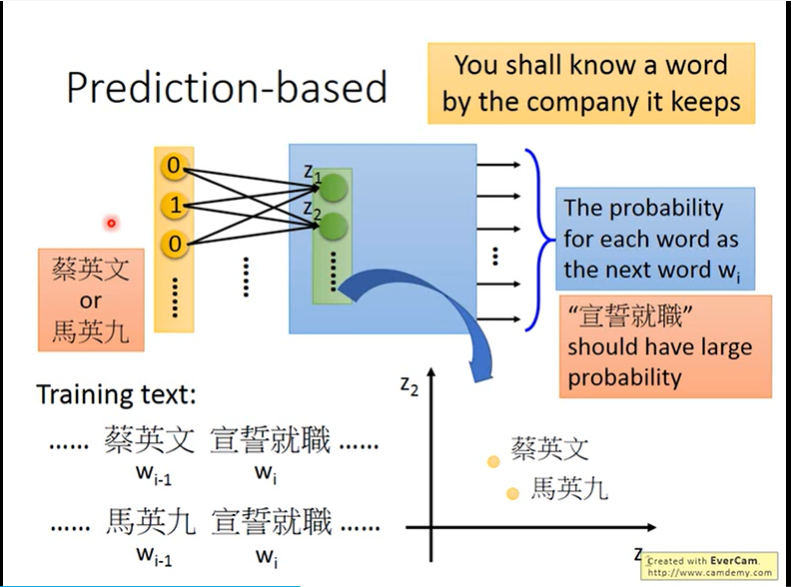
\includegraphics[width=0.7\textwidth]{fig/prediction_based.png} %插入图片,[]中设置图片大小,{}中是图片文件名
        \caption{prediction based的方法示意图} %最终文档中希望显示的图片标题
        \label{prediction_based} %用于文内引用的标签
    \end{figure}

    \begin{figure}H]
        \centering %图片居中
        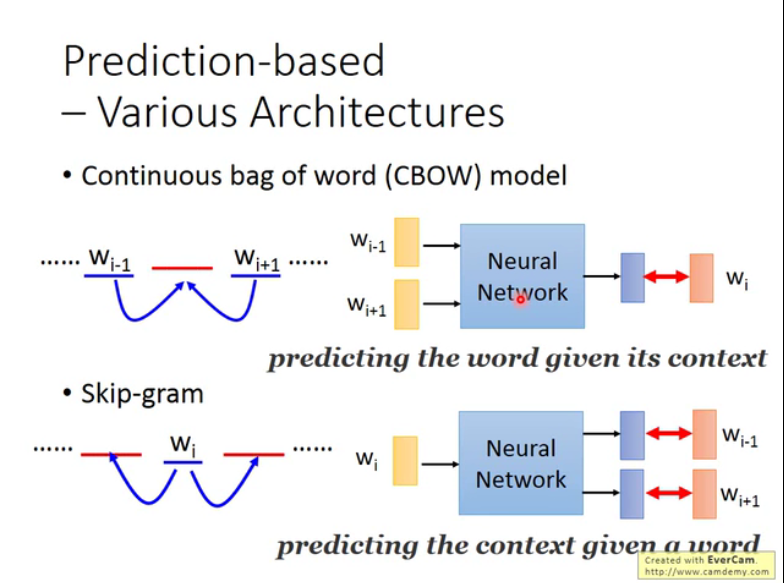
\includegraphics[width=0.7\textwidth]{fig/cbow_and_skip.png} %插入图片,[]中设置图片大小,{}中是图片文件名
        \caption{词袋模型和skip gram模型示意图} %最终文档中希望显示的图片标题
        \label{cbow_and_skip} %用于文内引用的标签
    \end{figure}
现在用的方法 Continuous bag of word(CBOW) model、Skip-gram。词袋模型是知道前后context单词去预测中间单词。skip gram是知道中间单词去预测前后单词。注意图中的Neural Network中不是DNN,原文中只是一个最简单的linear。
\end{itemize}
\subsection{一些有意思的事情}

\begin{itemize}
\item 左图是首都和国家之间的关系,可以发现这个关系在不同国家和首都之间存在一些共性,有点TransE的味道。右图是单词的不同时态之间的关系。
\begin{figure}[H]
    \centering
    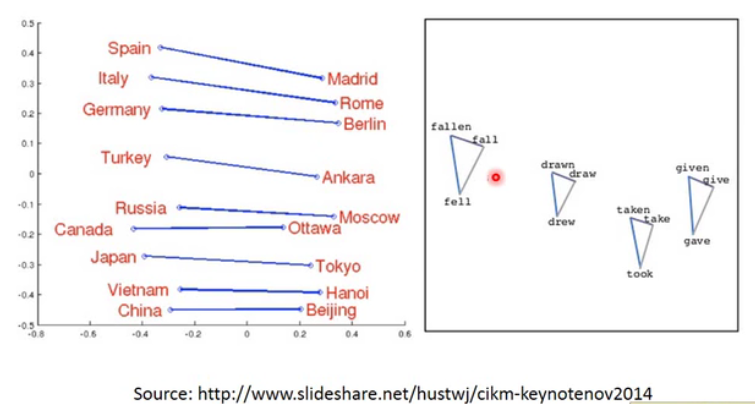
\includegraphics[width=0.7\textwidth]{fig/TransE.png}
    \caption{词和词之间的关系}
\end{figure}

\item 
\end{itemize} 在做图像分类时,对于机器没有见过的类别,模型往往不能得到正确的分类。例如在训练的时候只给了狗,汽车,马的图片,那么模型将无法将图片分类成猫。但是如果将图片和文字映射到同一个space下面,并且让对应的图片的embedding分布在对应的词语附近,那么只要知道了cat的位置,模型就有很大可能会把猫的图片放在cat这个词的附近,就能知道新图片的分类。
\begin{figure}[H]
    \centering
    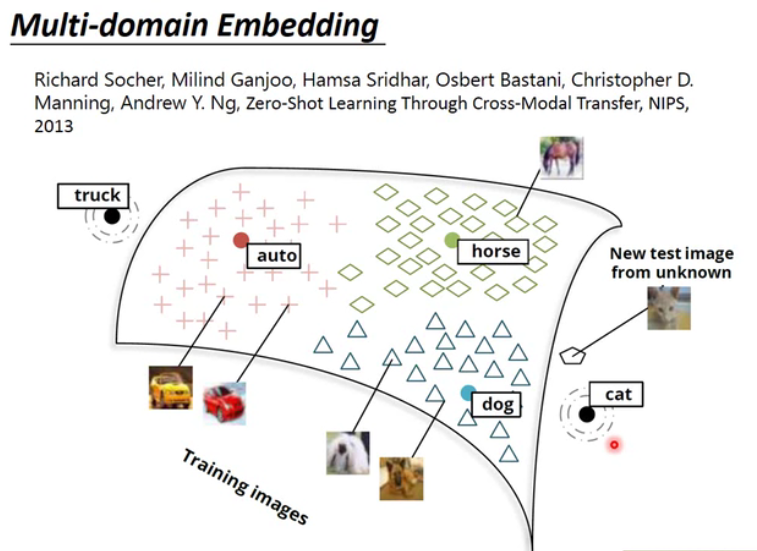
\includegraphics[width=0.7\textwidth]{fig/zero shot.png}
    \caption{多模态,有点zero shot的意思}
\end{figure}




\section{事件抽取}
\subsection{什么是时间抽取?}
事件抽取是从描述事件信息的文本中,识别并抽取出事件信息,并以结构化的形式呈现出来,包括发生的时间、地点、参与角色以及与之相关的动作或者状态的改变。
\begin{itemize}
    \item \textbf{事件描述(Event Mention)}:描述事件的词组/句子/句群,包含一个 trigger 以及任意数量的 arguments.
    \item \textbf{事件触发(Event Trigger)}:事件描述中最能代表事件发生的词汇,决定事件类别的重要特征,一般是动词或者名词
    \item \textbf{事件元素(Event Argument)}:事件的重要信息,或者说是实体描述(entity mention),主要由实体、属性值等表达完整语义的细粒度单位组成
    \item \textbf{元素角色(Argument Role)}:事件元素在事件中扮演的角色,事件元素与事件的语义关系,可以理解为 slot
    \item 事件类型(Event Type)
\end{itemize}
事件抽取基础任务是在 mention 中抽取一个 trigger 和多个 arguments,并找到每个 argument 对应的 role,以及 trigger 的 type。因此基础方法可以分成四步:
\begin{enumerate}
    \item Trigger Identification
    \item Trigger Type Classification
    \item Argument Identification
    \item Argument Role Classification
\end{enumerate}
\subsection{常用的方法}
\subsubsection{基于模式匹配}
\subsubsection{基于传统机器学习}
\subsubsection{基于深度学习}

\end{document}
